\apendice{Especificación de diseño}

\section{Introducción}\label{diseño}
En este apéndice se recoge el diseño de las interfaces, como se resolvieron los requisitos funcionales anteriormente expuestos~\pageref{requisitos}, el manejo de los datos o la estructura de los mismos.

\section{Diseño de datos}
En el tratamiento de los datos, se ha optado por hacerlo de dos formas diferentes, esto es debido, a que se necesita persistencia local y externa. Dependiendo de eso, tenemos dos diseños de datos diferentes.

\begin{itemize}
	\item \textbf{FireStore:} es la base de datos integrada en Firestore. Esta no sigue el modelo clásico, ya que es noSQL~\cite{wiki:nosql}, es decir, al igual que mongoDB~\cite{wiki:mongodb}, esta se gestiona mediante ficheros \emph{.json}. A diferencia SGBDR (Sistema gestor de bases de datos relacionales), la manera de trabajar de Firestore, es mediante un modelos no relacionales. Esta fue usada para la persistencia externa de datos. Como se puede ver en la siguiente imagen~\ref{fig:firestore} de la consola de Firebase:
	
	\begin{figure}[H]
		\centering
		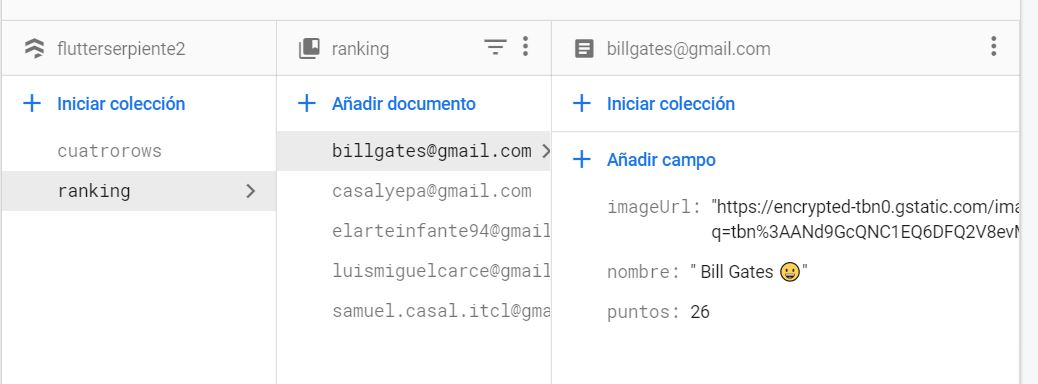
\includegraphics[width=0.9\textwidth]{disenio/firestore.jpg}
		\caption{Base de datos en firestore}\label{fig:firestore}
	\end{figure}

	\item \textbf{Sqlflite:} esta base de datos si que sigue el modelo tradicional del SGBDR. En mi caso fue necesario usar este paquete~\cite{package:sqlflite}, que internamente funciona con sqlite. Usado para almacenar datos en forma local, ya que no era necesario que los datos salieran del terminal. Una de las cosas a tener en cuenta de esto, es que si el usuario borra la caché de la aplicación o la desinstala se borran los ficheros correspondientes. Esto no debe de ser problema, ya que solo queremos almacenar ciertos valores.
	
\end{itemize}

\subsection{Diagrama entidad relación}
\begin{itemize}
	\item \textbf{FireStore:} la distribución en la base de datos es mediante colecciones, ver imagen~\ref{fig:diagramfirestore}. Como ejemplo podemos tener la colección para almacenar los datos del ranking, y para cada una de las entradas del ranking un fichero \emph{.josn} que haga referencia a los datos de cada usuario. Aunque esta no siga el modelo relacional, si que se podría implementar un diagrama entidad-relación, pero no se hace, porque es similar a tener dos tablas (colecciones en este caso) en la base de datos y que no tiene relación entre sí.
	
	\begin{figure}[H]
		\centering
		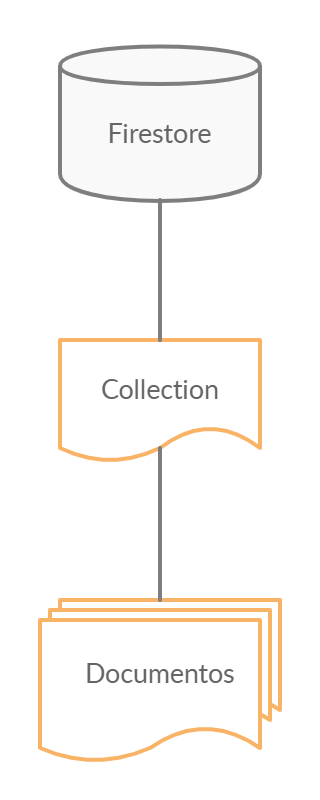
\includegraphics[height=0.9\textwidth]{disenio/diagramafirestore.jpg}
		\caption{Diagrama BD firestore}\label{fig:diagramfirestore}
	\end{figure}

	Una vez sabemos como es el funcionamiento de la base de datos noSQL, las dos colecciones necesarias para la aplicación fueron:
	
	\begin{itemize}
		\item \textbf{ranking:} se encarga de almacenar la mejor puntuación de cada uno de los jugadores del snake~\ref{fig:rankingexample}. Para distinguir cada uno de los documentos, se usa como clave primaria el correo del usuario, que también será el nombre que identifique a cada uno de estos ficheros.
		
		Las variables que almacena son: nombre(String), imagenUrl(String) y puntuación(int). 
		
		\begin{figure}[H]
			\centering
			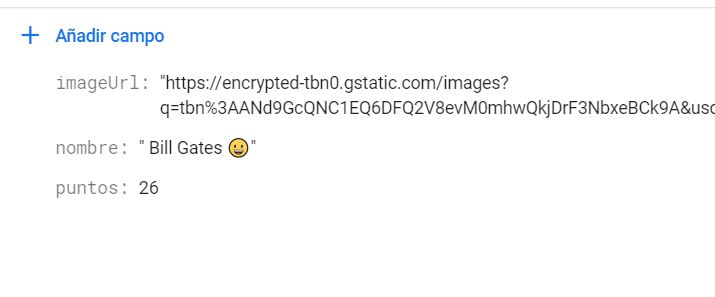
\includegraphics[width=0.9\textwidth]{disenio/rankingexample.jpg}
			\caption{Contenido json de rankinig}\label{fig:rankingexample}
		\end{figure}
	
		\item \textbf{cuatrorows:} esta colección guarda cada una de las partidas online del juego cuatro en raya~\ref{fig:cuatrorowsexample}. Los nombres de los documentos se generan de manera única en la base de datos, por lo que no puede haber dos partidas iguales.
		
		Por lo que la \emph{key} compartida durante el juego es la misma que el nombre del documento, dentro de esta colección. Los campos que tiene este documentos son muchos y variados, pero los más destacados son: 
		
		\begin{itemize}
			\item Posición de cada una de las fichas, de tipo String, y los valores que toma son Y, R o \emph{null}, dependiendo de la ficha que se encuentre en la celda.
			\item Datos de los jugadores de la partida, nombre, imagenUrl, correos ... Todos de tipo String.
			\item Flags para controlar si se producen ciertos eventos, como puede ser el final de la partida, si se ha mostrado el mensaje, lanzamiento de la moneda para el sorteo de quien inicia o el mensaje escrito por cada uno de los jugadores. Todas ellas son de tipo String, exceptuando las que puedan tomar valores de verdadero o falso.
		\end{itemize}
	
		\begin{figure}[H]
			\centering
			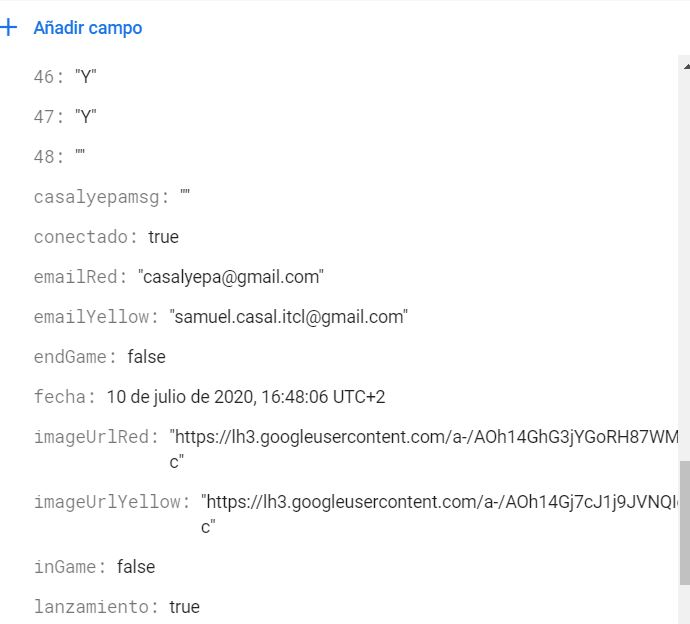
\includegraphics[width=0.9\textwidth]{disenio/cuatrorowsexample.jpg}
			\caption{Contenido json de cuatorows}\label{fig:cuatrorowsexample}
		\end{figure}
	\end{itemize}
	
	\item \textbf{Sqlflite:}
	
\end{itemize}
\section{Diseño procedimental}

\section{Diseño arquitectónico}


